\documentclass[12pt]{article}

%%%%%%%%%%%%%%%%%%%%%%%%%%
%%%  COMMON PACKAGES  %%%%
%%%%%%%%%%%%%%%%%%%%%%%%%%

\usepackage{amsmath}
\usepackage{amssymb}
\usepackage{amsfonts}
\usepackage{graphicx}
\usepackage[utf8]{inputenc}
\usepackage{amsthm}

%%%%%%%%%%%%%%%%%%%%%%%%%%%%%%%%%
%%%  UNUSUAL PACKAGES        %%%%
%%%  Uncomment as necessary. %%%%
%%%%%%%%%%%%%%%%%%%%%%%%%%%%%%%%%

%% MATH AND PHYSICS SYMBOLS
%% ------------------------
\usepackage{slashed}       % \slashed{k}
\usepackage{mathrsfs}      % Weinberg-esque letters
\usepackage{pifont}        % check marks
\usepackage{bbm}           % \mathbbm{1} 
%\usepackage[normalem]{ulem} % for \sout
\usepackage{cancel}


%% CONTENT FORMAT AND DESIGN
%% -------------------------
\usepackage[dvipsnames]{xcolor}
\usepackage{fancyhdr}		% to put preprint number
\usepackage{lipsum}         % block of text 
\usepackage{framed}         % boxed remarks
\usepackage{subcaption}     % subfigures
\usepackage{cite}           % group cites
%\usepackage{tocloft}       % Table of Contents	
\usepackage{xspace}			% spacing after macros
\usepackage{listings}       % code environment	
\lstset{
		basicstyle=\ttfamily\footnotesize,
		breaklines=true,
		backgroundcolor=\color{gray!15!white}}


%% TABLES IN LaTeX
%% ---------------
\usepackage{booktabs}      % professional tables
\usepackage{nicefrac}      % fractions in tables,
\usepackage{multirow}      % multirow elements 
\usepackage{arydshln} 	    % dashed lines in arrays

%% Other Packages and Notes
%% ------------------------
\usepackage[font=small]{caption} % small capt font
\usepackage{float}         % for strict placement e.g. [H]


%% CUSTOM PACKAGES
%% ---------------
\usepackage{tikzfeynman}   % Flip's rules Feynman Diagrams



%%%%%%%%%%%%%%%%%%%%%%%%%%%%%%
%%%  DOCUMENT PROPERTIES  %%%%
%%%%%%%%%%%%%%%%%%%%%%%%%%%%%%
\usepackage[margin=2cm]{geometry}   % margins
\graphicspath{{figures/}}			% figure folder
\numberwithin{equation}{section}    % set equation numbering


%% References in two columns, smaller
%% http://tex.stackexchange.com/questions/20758/bibliography-in-two-columns-section-title-in-one
\usepackage{multicol}
\usepackage{etoolbox}
\usepackage{relsize}
\patchcmd{\thebibliography}
  {\list}
  {\begin{multicols}{2}\smaller\list}
  {}
  {}
\appto{\endthebibliography}{\end{multicols}}


% Change list spacing
% from: http://en.wikibooks.org/wiki/LaTeX/List_Structures#Line_spacing
\let\oldenumerate\enumerate
\renewcommand{\enumerate}{
  \oldenumerate
  \setlength{\itemsep}{1pt}
  \setlength{\parskip}{0pt}
  \setlength{\parsep}{0pt}
}

\let\olditemize\itemize
\renewcommand{\itemize}{
  \olditemize
  \setlength{\itemsep}{1pt}
  \setlength{\parskip}{0pt}
  \setlength{\parsep}{0pt}
}


%%%%%%%%%%%%%%%%%%%%%%%%%%%
%%%  (RE)NEW COMMANDS  %%%%
%%%%%%%%%%%%%%%%%%%%%%%%%%%

%% FOR `NOT SHOUTING' CAPS (e.g. acronyms)
%% ---------------------------------------
\newcommand{\acro}[1]{\textsc{\MakeLowercase{#1}}}    

%% COMMON PHYSICS MACROS
%% ---------------------
\renewcommand{\tilde}{\widetilde}   % tilde over characters
\renewcommand{\vec}[1]{\mathbf{#1}} % vectors are boldface
\newcommand{\dbar}{d\mkern-6mu\mathchar'26}    % for d/2pi
\newcommand{\ket}[1]{\left|#1\right\rangle}    % <#1|
\newcommand{\bra}[1]{\left\langle#1\right|}    % |#1>
\newcommand{\Xmark}{\text{\sffamily X}}        % cross out

%% COMMANDS FOR TEMPORARY COMMENTS
%% -------------------------------
\newcommand{\comment}[2]{\textcolor{red}{[\textbf{#1} #2]}}
\newcommand{\flip}[1]{{
	\color{green!50!black} \footnotesize [\textbf{\textsf{Flip}}: \textsf{#1}]
	}}


%% COMMANDS FOR TOP-MATTER
%% -----------------------
\newcommand{\email}[1]{\href{mailto:#1}{#1}}
\newenvironment{institutions}[1][2em]{\begin{list}{}{\setlength\leftmargin{#1}\setlength\rightmargin{#1}}\item[]}{\end{list}}


%% COMMANDS FOR LATEXDIFF
%% ----------------------
%% see http://bit.ly/1M74uwc
\providecommand{\DIFadd}[1]{{\protect\color{blue}#1}} %DIF PREAMBLE
\providecommand{\DIFdel}[1]{{\protect\color{red}\protect\scriptsize{#1}}}

%% REMARK: use latexdiff option --allow-spaces
%% for \frac, ref: http://bit.ly/1iFlujR




%%%%%%%%%%%%%%%%%%%%%%%%%%%%%
%%% Theorem Environments %%%%
%%%%%%%%%%%%%%%%%%%%%%%%%%%%%

\newtheorem{theorem}{Theorem}[section]			
\newtheorem{lemma}[theorem]{Lemma}				
\newtheorem{corollary}[theorem]{Corollary}		
\newtheorem{fact}[theorem]{Fact}
\newtheorem{remark}[theorem]{Remark}

\theoremstyle{definition}						
\newtheorem{definition}[theorem]{Definition}	
\newtheorem{claim}[theorem]{Claim}	
\newtheorem{eg}[theorem]{Example}






%%%%%%%%%%%%%%%%%%%%%%%%%%%%%%%%%%%%%%%%%%%%%%
%%%  TIKZ COMMANDS FOR EXTERNAL DIAGRAMS  %%%%
%%%  requires -shell-escape               %%%%
%%%  in texpad 1.7: prefs > shell esc sec %%%%
%%%%%%%%%%%%%%%%%%%%%%%%%%%%%%%%%%%%%%%%%%%%%%

%% For exporting tikz figures as into a ./tikz/ subfolder.
%% It is useful if you want pdf versions of the tikz diagrams or
%% if you need to speed up compilation of a large document with
%% many tikz diagrams.

%\write18{} % Careful with this!
%\usetikzlibrary{external}
%\tikzexternalize[prefix=tikz/] % folder for external pdfs


%%%%%%%%%%%%%%%%%%%
%%%  HYPERREF  %%%%
%%%%%%%%%%%%%%%%%%%

%% This package has to be at the end; can lead to conflicts

\usepackage[
	colorlinks=true,
	citecolor=green!50!black,
	linkcolor=NavyBlue!75!black,
	urlcolor=green!50!black,
	hypertexnames=false]{hyperref}


%%%%%%%%%%%%%%%%%%%%%
%%%  TITLE DATA  %%%%
%%%%%%%%%%%%%%%%%%%%%

%% PREPRINT NUMBER USING fancyhdr
%% Don't forget to set \thispagestyle{firststyle}
%% ----------------------------------------------
\renewcommand{\headrulewidth}{0pt} 	% no separator
\setlength{\headheight}{15pt} 		% min to avoid fancyhdr warning
\fancypagestyle{firststyle}{
	\rhead{\footnotesize%
%	\texttt{UCI-TR-2016-XX}\\ %% Uncomment for additional preprint #s
	\texttt{UCR-PHYS-165-W2018-A}%
	}}

%% TOC overwrites fancyhdr, here's a fix
%% http://tex.stackexchange.com/questions/167828/difficult-with-fancyhdr-and-table-of-contents
\usepackage{etoc}
\renewcommand{\etocaftertitlehook}{\pagestyle{plain}}
\renewcommand{\etocaftertochook}{\thispagestyle{firststyle}}



\begin{document}

%\thispagestyle{empty}		% default if no preprint #
\thispagestyle{firststyle} 	% to include preprint

\begin{center}

    {\huge \bf P165: Introduction to Particle Physics}

    \vskip .7cm

%% SINGLE AUTHOR FORMAT
%% --------------------
	Prof.~\textbf{Flip Tanedo} %\\
	(\texttt{\footnotesize \email{flip.tanedo@ucr.edu}})

	\vspace{-1em}
    \begin{institutions}[2.25cm]
    \footnotesize
    {\it 
	    Department of Physics \& Astronomy, 
	    University of  California, Riverside, 
	    {CA} 92521	    
	    }    
    \end{institutions}


\end{center}




%%%%%%%%%%%%%%%%%%%%%
%%%  ABSTRACT    %%%%
%%%%%%%%%%%%%%%%%%%%%

\begin{abstract}
\noindent 
These are course notes for Physics 165.
%
\\
\textbf{These notes are in progress}. Last update: \today
\end{abstract}



\small
\setcounter{tocdepth}{2}
\tableofcontents
\normalsize
%\clearpage


%%%%%%%%%%%%%%%%%%%%%
%%%  THE MEAT    %%%%
%%%%%%%%%%%%%%%%%%%%%

%% Use \input if you have separate files.
%% \include is `smarter' (creates separate aux files
%% for each tex file) and hence more efficient, 
%% but it automatically puts a page break
%% between included files. Input doesn't do this.

\section{Contributions}

I appreciate \LaTeX\, contributions to these notes from the following students: 
%
Louis Penafiel % Week 1
.
These contributions are especially helpful for including the spontaneous discussion topics in class.

\section{Review of Preliminaries}

Our strategy for this course is to present the Standard Model by going over it multiple times, refining ideas and building up the theory. We're going to start off requiring only pop-level ideas in relativity and quantum mechanics---but you should read this section as a reminder of the `big picture' of your more technical studies in these topics.

\subsection{Units}
% Lecture 1

We work in \textbf{natural units}\footnote{For a very nice reference, see Jaffe's \acro{MIT} Quantum Theory Notes: Natural Units, \url{https://stuff.mit.edu/afs/athena/course/8/8.06/spring08/handouts/units.pdf}}. This means that we will measure everything in units of electron volts, usually MeV or GeV. The rule for natural units is:
\begin{align}
	\hbar = c = 1 \ .
\end{align}
How can this be? If you open up the \acro{PDG} particle booklet (``the \acro{PDG}'') to their table of constants, you'll find that
\begin{align}
	c & = 3 \times 10^8~\text{m}/\text{s}
	\\
	\hbar &= 7 \times 10^{-22}~\text{MeV~s} \ .
\end{align}
This means that if $c=1$, we can write
\begin{align}
	\text{second} = 3\times 10^8 \, \text{meter} \ ,
\end{align}
which is precisely what we mean by a \emph{light second}: the distance something would travel if it were traveling at the speed of light. 

Why is this useful? If you're driving from Riverside to Irvine at rush hour, you'd be happy to hit 20 mph. Why don't we define ``natural on the highway 91'' units where $c_\text{hwy 91} = 20~\text{mph}$ is used.

\begin{eg}
Han Solo claims to have done the Kessel Run in 12 parsecs. For most Star Wars fans, this doesn't make any sense: a parsec is a unit of distance, and Solo used it in place of a unit time. However, the relation $c=1$ gives us a way to show how to convert one type of unit to another. The trick is to just multiply by one in a useful way:
\begin{align}
	12\,\text{pc}
	= 12 \times 3 \times 10^{16}\,\text{m}\times (1/c)
%	\\
	= 4\times 10^{17}\, \text{m}
	\times\left(\frac{1}{3\times 10^{8}\,\text{m}/\text{s}}\right)
%	\\
	= 10^9\, \text{s} \ .
\end{align}
How did we know that 1~pc$= 3\times 10^{18}~$m? We looked it up in the \acro{PDG}. By the way, $10^9$ seconds is not particularly impressive---that's 30 years! $\blacksquare$
\end{eg}

Similarly, the relation $\hbar = 1$ lets us convert between energy and time. A good mnemonic of this is the Heinsenberg uncertainty principle, $\Delta E \Delta t\sim \hbar$, or otherwise the canonical commutation relation $[\hat E, \hat t] = i\hbar$. 

\begin{eg}The Large Hadron Collider smashes together protons at an energy of about 10 TeV. This corresponds to an inverse time, which by $c=1$ we can convert into an inverse length scale. We can find the value of this length scale in meters by ``multiplying by one'' to convert unis:
\begin{align}
	10~\text{TeV} \times
	\left(\frac{1}{7\times 10^{22}\,\text{MeV}\,\text{s}}\right)
	\times\left(\frac{1}{3\times 10^{8}\,\text{m}/\text{s}}\right)
	= 
	\frac{1}{10^{-20}\,\text{m}} \ .
\end{align}
The size of an atom is about an Angstrom, which is $10^{-10}~$m. From this we may guess that the \acro{LHC} probes length scales $10^{10}$ times smaller than an atom. This turns out to be too na\"ive---we'll see why in this class---but the principle is clear: high-energy colliders are \emph{microscopes}. The higher the energy, the smaller the length scale being probed. This is why particle physics is also known as \textbf{high-energy physics}. 
	$\blacksquare$
\end{eg}

\begin{eg}
Sidney Coleman\footnote{\url{https://www.physics.harvard.edu/events/videos/Phys253}} described natural units by saying that swinging your arms around has microscopic velocity and astronomical  angular momentum.
\end{eg}

%For more background on this, see Jaffe's \acro{MIT} notes on units.



\subsection{Kinematics}
% Lecture 1

\textbf{Kinematics} has to do with how we describe motion. Since we're going to high energies, it is important to include the effects of special relativity. You should be familiar with four-vectors and Lorentz transformations---we will be using them later in these lectures. For now, however, we're going to limit ourselves to three useful rules:
\begin{enumerate}
	\item Energy is conserved in any process.
	\item Momentum is conserved in any process.
	\item The Einstein relation,
\begin{align}
	E^2 = m^2 + \vec{p}^2 \ .
\end{align}
\end{enumerate}
%
Recall that the first two rules come from the invariance of special relativity with respect to time translations and space translations, respectively. We will assume these features in this course, but it may be worth remembering that our universe is decidedly not time-translation invariant: this is why photons from the cosmic microwave background are \emph{red-shifted}: they lose energy as the universe expands.

The Einstein relation is the relativistic version of the famous $E=mc^2$. Those with a mathematical inclination may want to read this as
\begin{align}
	m^2 = E^2 - \vec{p}^2 \ ,
	\label{eq:mass:shell}
\end{align}
which is nice because it describes an invariant (mass) in terms of the Lorentz norm of the momentum four-vector, $p^2 = E^2-\vec p^2$ where $p_\mu = (E, \vec p)$. By the way, by writing this we have chosen the `mostly-minus' metric. This is a convenient choice because it means that squared particle masses are positive. We'll dig more deeply into four-vectors as we progress. 

It is useful to introduce some nomenclature. A particle whose energy and momenta satisfies the Einstein relation is said to be \textbf{on-shell}. In contrast, a particle that is \emph{not} on-shell is called \textbf{virtual} (or, equivalently \textbf{off-shell}). This should sound strange! We just said that the Einstein relation is a rule---why should we separate particles into those that do and do not obey the rule? The answer is that particle physics is a quantum theory, and not all quantum particles are on-shell.

\begin{eg}
The terminology \emph{on-shell} is somewhat silly. The idea is that if you imagine a particle, it can have a continuum of different values of energy and momentum depending on what reference frame you're in. If you go from the rest frame to any other frame, the particle picks up momentum. If you rotate, the momentum is shifted from one set of components to another. The mass shell condition (\ref{eq:mass:shell}) is a restriction on the four-dimensional space of possible momenta, $(E,\vec p)$. That restriction says that \emph{no matter what reference frame you're in, this particle exists somewhere on this surface}. If you imagine that surface as a `shell' in the four-dimensional space, then you arrive at the curious nomenclature. $\blacksquare$	
\end{eg}


\subsection{Special Relativity}

It is convenient to combine kinematic variables into \textbf{four-vectors},
\begin{align}
	p_\mu = \begin{pmatrix}
		E,&
		p_x,&
		p_y,&
		p_z&
	\end{pmatrix} \ .
\end{align}
You can ``divide by one'' by writing $E\to E/c$ if you want to go to casual units. You can also write coordinates as objects with four components, $x^\mu = (t,x,y,z)$. The Greek index $\mu$ is used to index the four components of a vector. They remind us that these components transform into one another under Lorentz transformations. 

We use the \emph{mostly-minus} convention for the metric,
\begin{align}
	\eta_{\mu\nu} = \eta^{\mu\nu} = \begin{pmatrix}
		 1 &&& \\
		& -1 &&\\
		&& -1 &\\
		&&& -1 \\
	\end{pmatrix} \ .
\end{align}
This is a rule for contracting indices. An object that has no free indices is a scalar, which means that it does not change when you do a Lorentz transformation---that is, when you change reference frames. 

\begin{eg} The `square' of the four-momentum is
	\begin{align}
	p^2 = p\cdot p = p^\mu p_\mu = \eta^{\mu\nu} p_\nu p_\mu  \equiv m^2 \ . 	
	\label{eq:p2:m2}
	\end{align}
\end{eg}
Lorentz transformations, $\Lambda^\mu_{\phantom{\mu}\nu}$ are two-index objects that act on four-vectors. The whole point of special relativity is that we can model our universe as Minkowski space: a four-dimensional space that is the obvious generalization of three-dimensional Euclidean space \emph{except} for a curious minus sign in how we define dot products.

If you need a refresher on some of these topics, I recommend the following:
\begin{itemize}
	\item Everything you need to know about special relativity is in a charming little book by Sander Bais, \emph{Very Special Relativity}. It doesn't look like a technical book (it's not), but you'll review everything you need to know.
\end{itemize}

\subsection{Quantum Mechanics}
% lecture 2

Particle physics is inherently quantum.
%
You should already have some formal training in quantum mechanics. Rather than re-hashing formalism, we can review all of the key ideas recalling some the favorite `pop physics' quantum mechanics examples. I leave it to you to review the formalism as necessary---in this course we will need a familiarity with quantum mechanics at the level of Griffiths' textbook. The more background you have the better, especially understanding the underlying linear algebra of quantum mechanics.

\begin{eg}
The `quantum' in quantum mechanics means discrete. You know that the energy levels of hydrogen being discretized (and hence \emph{chemistry}). You also know that things like angular momentum with respect to some axis. But not everything is quantized: the free particle has a continuum of allowed energies and momenta. What's the difference between a free electron and one in the hydrogen atom? 
%
The marriage of quantum mechanics and special relativity introduces a new sense of quantization: we quantize in the \emph{number of particles}. For rather curious reasons, this is historically called \emph{second quantization}, though the terminology has rightfully fallen out of favor.  $\blacksquare$
\end{eg}


\subsubsection{Schr\"odinger's cat}

Schr\"odinger's cat is placed in a box along with some dangerous cat-killing device that is triggered by the radioactive decay of a single uranium nucleus. You directly observe the cat as you close the box, and then some time later you open up the box again. When you observe the cat once again, you can confirm that it is either alive or dead. Quantum mechanics tells us that in between these direct observations, the cat  is in a superposition of alive and dead.

What do we get out of this? Here's one glib interpretation: the states that we observe make sense classically. The things that our experiments produce are \emph{observations}. Quantum mechanics ``happens'' \emph{in between} observations. 

\subsubsection{The double slit experiment}

To clarify what we mean by `in between' observations, we can turn to another important example in quantum mechanics: the double slit experiment. \flip{insert image, describe experiment.}

It is not simply that the particle took one path or another but we don't know.
%
The particle takes both paths to travel from its initial observed position $|\text{in}\rangle$ to reach its [observed] detection point $|\text{out}\rangle$. 
%
How do we know this? Each path is associated with a complex number, for example let us write
\begin{align}
		\langle \,\text{out}\, |  \,1 \,\rangle
		\langle \, 1\, |  \,\text{in} \,\rangle
		&&
		\text{and}
		&&
		\langle \,\text{out}\, |  \,2 \,\rangle
		\langle \, 2\, |  \,\text{in} \,\rangle
\end{align}
to be the amplitudes for the particle take the first slit and second slit, respectively.  The total amplitude can be understood mathematically by inserting a \emph{complete set of intermediate states}, which is a fancy way of inserting the identity matrix:
\begin{align}
	\langle \text{out} | \text{in}\rangle
	 = 
	\sum_{a}^{1,2}
	\langle \,\text{out}\, |  \, a \,\rangle
		\langle \, a\, |  \,\text{in} \,\rangle \ .
	\label{eq:double:slit:sum}
\end{align}
The probability for this process is $|\langle \text{out} | \text{in}\rangle|^2$. The relative phase of the terms in the sum determines the interference between the two paths. The existence of the interference patterns on the screen is a smoking gun that both paths are being sampled.
%
We can make this more explicit by inserting the matrix identity in the following way:
%
Sometimes this is called a `sum over histories.'  

The key point to remember here is this: the amplitude to go from one observed initial state to an observable final state is given by the sum of the amplitudes for all possible ways in which the initial state can reach the final state. 


\subsubsection{An aside on dynamics}


We're being a rather glib about what we mean by the amplitude $\langle \text{out} | \text{in}\rangle$. You may raise the objection that the issue of time evolution is probably important: the `in' state ought to have happened \emph{before} the `out' state, and there should be some operator, $\exp(-iHt)$, that acts on states to evolve them in time. You would be absolutely correct, and you could dress up (\ref{eq:double:slit:sum}) by inserting these time evolution operators explicitly. You might end up with something like this
\begin{align}
	\langle \text{out} | \text{in}\rangle
	 = 
	\sum_{t_i}
	\sum_{a}^{1,2}
	\langle \,\text{out}\, | e^{-iH(t_\text{out}-t_i)} | \, a \,\rangle
		\langle \, a\,  |  e^{-iH(t_i-t_\text{in})} |  \,\text{in} \,\rangle \ .
\end{align}
It all gets rather tedious and goes well beyond what we wanted to learn from our example\footnote{You may find it useful to read the introductory remarks in any standard quantum field theory book about canonical quantization and the choice of Heisenberg, Schr\"odinger, and ``interaction'' pictures for time evolution. But then you might as well keep reading and learn particle physics from the ground up, in which case you don't need these lectures because you'll have learned it all the hard way.}.

For now we do not care about the details. In fact, we only bring up the time evolution to make one useful point.  If you start with some particle configuration $\left|\text{in}\right\rangle$ and end up with some other later configuration $\left|\text{out}\right\rangle$, then all we can do is ask about
\begin{align}
	\langle \text{out} | (\text{time evolution}) | \text{in}\rangle \ ,
\end{align}
where ``(time evolution)'' refers to the time evolution operator. This operator encodes the \textbf{dynamics} of a theory and tells us about all possible allowed histories between the initial and final states. Everything that happens ``in between'' the initial and final states has to be summed over. In the same way that the interference pattern in the double slit experiment comes from summing the amplitudes of different paths, the amplitude $\langle \text{out} | (\text{time evolution}) | \text{in}\rangle $ involves a sum over all possible dynamics that aren't directly observed. 



\subsubsection{The $\infty$ slit experiment}

You can modify the double slit experiment. If you have three slits, then you sum the amplitudes for all three possible paths:
\begin{align}
	\langle \text{out} | \text{in}\rangle
	 = 
	\sum_{a=1}^{3}
	\langle \,\text{out}\, |  \, a \,\rangle
		\langle \, a\, |  \,\text{in} \,\rangle \ .
\end{align}
If you take that configuration, and then insert a second barrier which has, say, five slits, then:
\begin{align}
	\langle \text{out} | \text{in}\rangle
	 = 
	\sum_{a_1 = 1}^{3}
	\sum_{a_2 = 1}^{5}
	\langle \,\text{out}\, |  \, a_2 \,\rangle
	\langle \, a_2\, | \, a_1 \,\rangle
		\langle \, a_1\, |  \,\text{in} \,\rangle \ .
\end{align}
Now we have a sum over $3\cdot 5 = 15$ paths. We could go on ad infinitum, adding an \emph{infinite} number of barriers, but each with an \emph{infinite} number of slits. This seemingly absurd limit is really just the limit of there being empty space between the source and detector. The particle is free to go anywhere it pleases. The sum turns into a continuous integration over all possible paths between the source and detector.

This notion should be familiar to you from the principle of least action in classical mechanics. By minimizing the action, $\delta S = 0$, one obtains the Euler--Lagrange equations that determine the classical trajectory. This classical trajectory is precisely what satisfies Newton's laws. What's really weird is that this is a variational problem: somehow a classical particle knows to `sample' all possible paths, but the trajectory that it takes ends up being the one that minimizes $S$ over all of these paths. How does it know to sample these paths\footnote{This idea is integrated into science fiction very nicely in the short story, ``Story of your life'' by Ted Chiang, which has been converted into a film \emph{Arrival}, which unfortunately downplays the physics.}? This is an idea that we would like to explore further in these lectures. 




\subsubsection{Scattering}

 To study a subatomic particle, one does not simply\footnote{\url{http://knowyourmeme.com/memes/one-does-not-simply-walk-into-mordor}} pick up a subatomic particle and look at it. To pull this into a classical analogy, what happens when you want to study an apple by looking at it?
\begin{center}
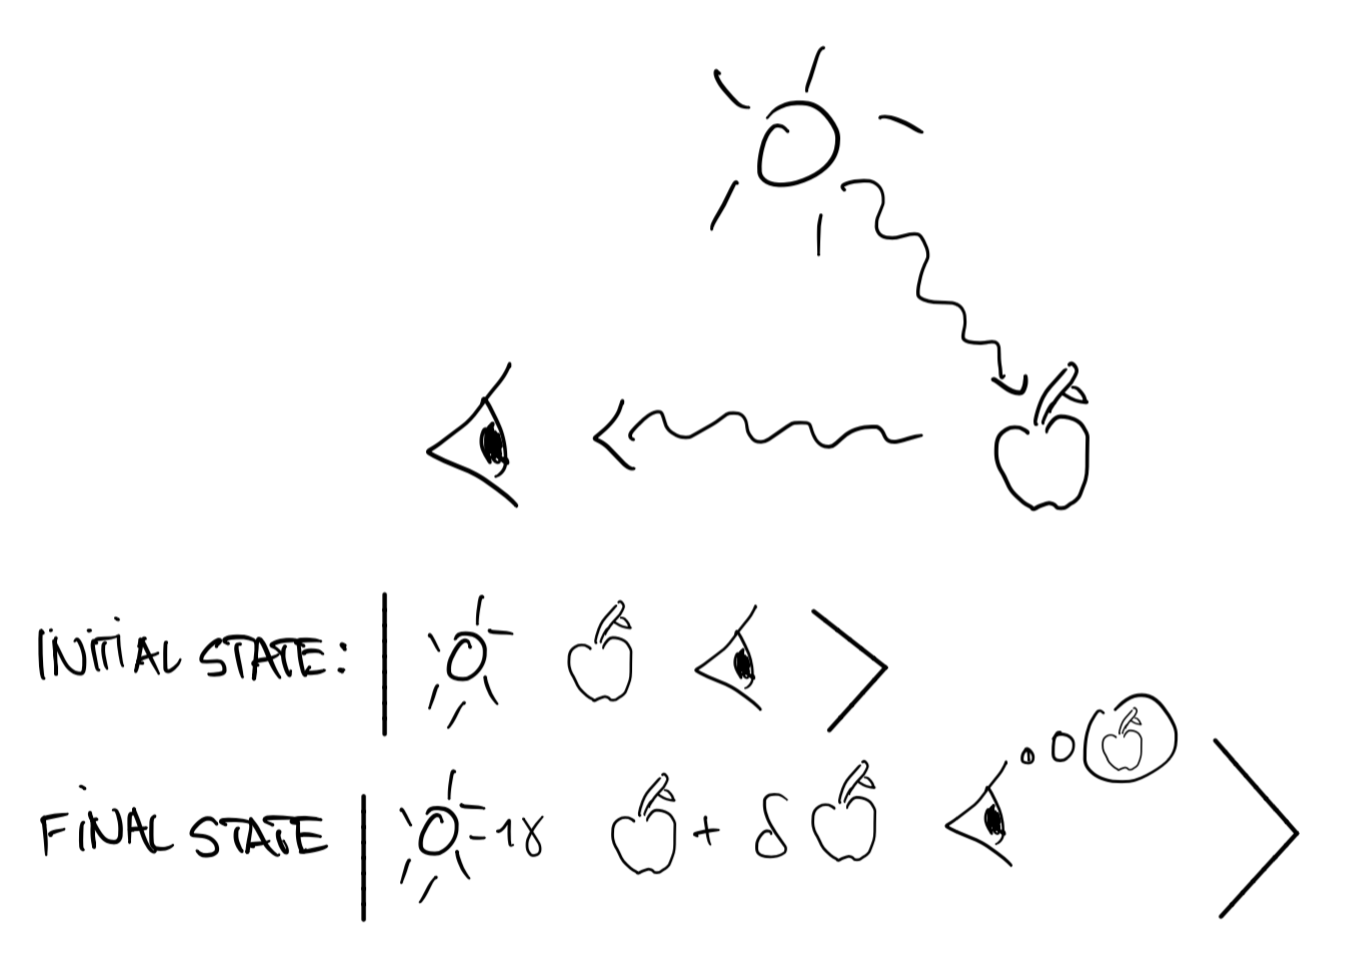
\includegraphics[width=.7\textwidth]{Lec1_lp_applescatter}	
\end{center}
Light from the sun strikes the apple, perhaps imparting some very small momentum. Then light from the apple bounces into your eyes, causing some series of neurological impulses that lead your consciousness to \emph{observe} the apple. This is a `scattering' process between an initial state and a final state. The initial state has the sun, the apple, and you. The final state has the same objects, though perhaps the sun is now a little less energetic because of the photon that it lost, the apple has picked up some small momentum, and you are now thinking about apples. This is, at its heart, a scattering process.

There are remarkably few particles that we can actually detect directly. These particles are reasonable $|\text{in}\rangle$ and $|\text{out}\rangle$ states. Most particles only exist in a fleeting moment in a quantum mechanical sense before turning into one or more objects---some of which eventually become detectable states. 
%
The punchline is that in this course, we will be focused on two kinds of quantum processes:
\begin{itemize}
	\item \textbf{Scattering}: a two or more particles go to a configuration of two or more particles.
	\item \textbf{Decays}: a single particle turns into two or more particles.
\end{itemize}
To simplify nomenclature, we will use \textbf{scattering} to refer to either type of process. We describe scattering processes using a graphical tool called \textbf{Feynman diagrams}; we will devote most of our time understanding what these are, how to draw them, and how to interpret them. 

\subsubsection{Amplitudes are complex numbers}

Most of these lectures will be spent thinking about scattering amplitudes. It is of critical important to internalize that these scattering amplitudes are nothing magical, they're simply complex numbers. We will postpone a discussion of how to calculate these numbers---you should take the graduate version of this course if you want to really do that carefully---but rather focus more on how Feynman diagrams capture the essence of these amplitudes. As we point to these diagrams and try to interpret them, \emph{do not fool yourself into thinking that this is some kind of shamanism}. At the end of the day, everything that we're doing is summing over complex numbers that each represent a path from an initial state to a final state.



\subsubsection{Ideas that we didn't use}

Let us make one more remark: in this section we've left out hundreds of pages of quantum mechanics that you can find in your favorite textbooks on the subject. One of the most notable omissions is the idea of a \textbf{wave function}. This is very deliberate. 

Wave functions are a nice segue to transition from classical to quantum mechanics. It gives you an object that makes it easy to ask `what is the probability that a particle is \emph{here}?' We even have a handy differential equation, the Schr\"odinger equation, to govern its evolution in time. However, this obfuscates the point that quantum mechanics is ultimately about \emph{linear algebra}, rather than differential equations. Further, the wave function \emph{looks a lot} like another object that we will need: the quantum field, which is very, very different. Wave functions are, at their core, states: $\Psi(\vec x) = |\vec x\rangle$. The quantum field, on the other hand, is an operator---it is a matrix that acts on the space of states. 





\section{Particle Physics}
\label{sec:preliminaries:particles}

A \textbf{model} is a theory of particle physics. We use this nomenclature for two reasons:
\begin{enumerate}
	\item It is a reminder that this is a human construction meant to approximate nature.
	\item It frees up the word `theory' for things like the ``theory of special relativity'' and ``quantum field theory,'' which are the mathematical super-structures that contain our models\footnote{All of our models are quantum field theories; quantum field theory is a general framework to describe models consistently.}.
\end{enumerate}
This isn't ``official'' in any way; I just made it up. Anyway, these are just words. 

For now let us define a \textbf{model} as being composed of two things:
\begin{enumerate}
	\item A list of particles.
	\item A list of interactions between particles. 
\end{enumerate}
In time we will refine these ideas. After all, we haven't said anything about fundamental forces or symmetries. For now, it is much more interesting to just dive right in and see what a model of particle physics looks like.

\subsection{Feynman Rules}

We define a model by listing the Feynman rules that govern how to draw valid Feynman diagrams for that model. These rules boil down to identifying a list of particles (and how to represent them) and how these particles are allowed to interact. Here's how it works.

\begin{itemize}
	\item \textbf{Particles}: A particle is represented by a line. These lines may have decorations to distinguish them from other types of particles, but the most important thing is that they are lines that connect two different points.
	\item \textbf{Interactions}: Some number of particles may \emph{interact} if their lines can come together into a vertex. This means each line connects to the same point. A list of allowed interactions are a list of allowed ways in which different lines can come together.
\end{itemize}


\section{Quantum electrodynamics}

As the name implies, \textbf{quantum electrodynamics} (\acro{QED}) is the marriage of classical electrodynamics (Maxwell's equations) and quantum mechanics. In fact, it is a little more than that: electrodynamics has special relativity built into it. So \acro{QED} is actually the combination of classical electrodynamics with \emph{relativistic} quantum mechanics. This latter discipline is called \textbf{quantum field theory} and is the theoretical underpinning of everything we're doing. Rather than build \acro{QED} from quantum field theory, we're going to take the approach of Section~\ref{sec:preliminaries:particles}. 

What you should be thinking right now is that classical electrodynamics was all about the \textbf{electromagnetic field}. You learned that ripples in this field travel at the speed of light and that this field is what mediates the electromagnetic force. Somewhere in the transition from classical electrodynamics to quantum electrodynamics, this field is \emph{quantized} and we get to talk about particles. In due course we will flesh out this skeleton of ideas with formalism---but suffice it to say that the {photon}, one of our key players in \acro{QED}, is indeed a quantum of the electromagnetic field\footnote{I'm already lying to you. Actually, a photon is a quantum of the electromagnetic potential, which you may recall is $A_\mu(x)$. Derivatives of this potential give the electromagnetic fields.}.

Our goal in this section is to develop a theory by defining its \textbf{Feynman rules}. These are rules for how to draw \textbf{Feynman diagrams}.

\subsection{The particles}

Quantum electrodynamics has two particles: the \textbf{electron}, $e$, and the \textbf{photon}, $\gamma$. If you want to be nit picky, the electron has negative charge so we should call it $e^-$ so that we know what charge it has. 



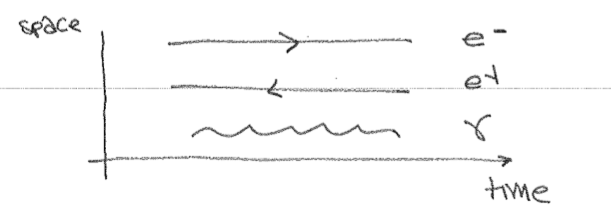
\includegraphics[width=\textwidth]{Lec1_forward}

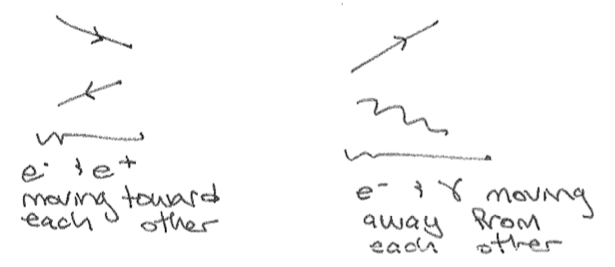
\includegraphics[width=.6\textwidth]{Lec1_noaxis}


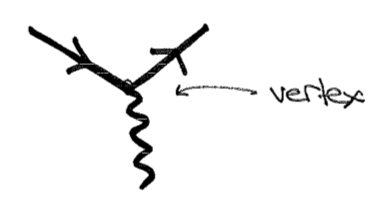
\includegraphics[width=.3\textwidth]{Lec1_vertex}

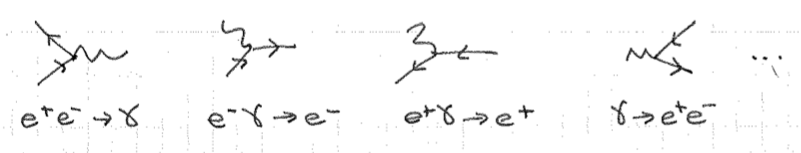
\includegraphics[width=\textwidth]{Lec1_3pt}

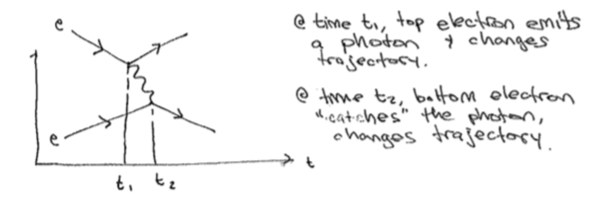
\includegraphics[width=\textwidth]{Lec1_order}


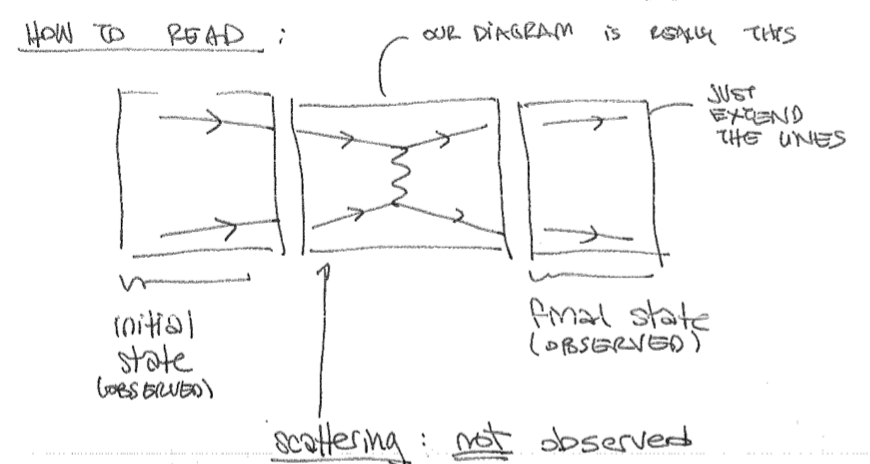
\includegraphics[width=\textwidth]{Lec1_diagram}

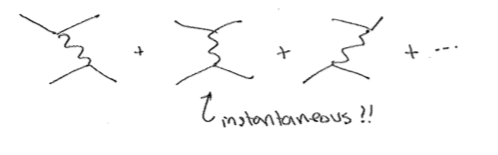
\includegraphics[width=\textwidth]{Lec1_sum}



\subsection{Conservation of Charge}



\section{Quantum Field Theory}

Why we have quantum fields: locality and causality. all of our feynman rules are local. Conservation of objects occurs locally. But there's something about the lines that are non-local. 

% phasors?
% what are we taylor expanding about 


\section{Particle Botany}

\begin{quote}
\emph{If I could remember the names of these particles, I would have been a botanist.}\\
	-- Enrico Fermi	(via Leon Lederman\footnote{\url{https://quoteinvestigator.com/2017/07/19/particles/}})
\end{quote}



\section*{Acknowledgements}


%
\textsc{p.t.}\ thanks 
\emph{your name here}
for useful comments and discussions. 
%
\textsc{p.t.} thanks the Aspen Center for Physics (NSF grant \#1066293) for its hospitality during a period where part of this work was completed.

%% Appendices
% \appendix


%% Bibliography
\bibliographystyle{utphys} 	% arXiv hyperlinks
% \bibliography{bib title without .bib}


\end{document}